% --- SOFT DELETE: Original Section 5 (Batch 4) ---
%
% \section{Use-Case–Driven Performance Evaluation}
% \label{sec:use-case}
%
% \tresumo{Avaliação e Resultados: Teste da infraestrutura provisionada através do caso prático utilizando o Star Schema Benchmark (SSB).}
%
% This chapter presents a practical test case designed to validate the provisioned infrastructure under a real-world 
% analytical scenario. To guide the technical evaluation, the analysis is conducted based on a central hypothesis: 
% in environments with severely restricted hardware, such as the free tier ARM instances utilised in this project, 
% the \emph{in-memory} processing capabilities of Apache Spark with caching will outperform the traditional 
% disk-allocated batch execution of Apache Hive. Formulating this hypothesis is essential for structuring the 
% benchmarking tests, allowing the obtained results to be directly compared against the initial architectural 
% predictions.
%
% \subsection{Experimental Methodology and Infrastructure Setup}
%
% The experimental procedure was modelled using the Star Schema Benchmark (SSB), enabling researchers 
% to reproduce the stress tests within their own cloud laboratories. The hardware allocation utilised 
% the predefined Terraform blueprints, specifically targeting the \texttt{data-science} profile.
%
% Following the \texttt{terraform apply} execution, the \emph{cluster} instantiated four nodes: 
% one \emph{master} and three \emph{worker} machines. Each node was provisioned as a 
% \texttt{VM.Standard.A1.Flex} instance, strictly limited to 1 OCPU and 6 GB of RAM. The active 
% services focused on the core components required for the benchmark: HDFS, YARN, Hive Metastore, 
% and Spark 3.
%
% \subsection{Data Ingestion and Hadoop Configuration}
%
% The ingestion phase commenced with the transfer of the SSB dataset, comprising a fact table and 
% multiple dimension tables in CSV format, to the secondary disk of the \emph{master} node. 
% Subsequently, the data was ingested into the Hadoop ecosystem to ensure visibility across the 
% distributed model of the \emph{cluster}. The physical size of the flat files injected into the 
% environment is detailed in Table~\ref{tab:ssb-dataset-sizes}, reflecting the storage baseline prior 
% to the HDFS block distribution.
%
% [tables, figures, queries, and remaining subsections omitted for brevity; see git history]
%
% --- END SOFT DELETE ---

%%%%%%%%%%%%%%%%%%%%%%%%%%%%%%%%%%%%%%%%%%%%%%%%%%%%%%%%%%%%%%%%%%%%%%%%%%%%%%%%%%%%%%%%%%%%%%%%%%%%%%%%%%%%%%%%%%
%%%%%%%%%%%%%%%%%%%%%%%%%%%%%%%%%%%%%%%%%%%%%%%%%%%%%%%%%%%%%%%%%%%%%%%%%%%%%%%%%%%%%%%%%%%%%%%%%%%%%%%%%%%%%%%%%%
%% REVISED Section 5 (Batch 4)
%%%%%%%%%%%%%%%%%%%%%%%%%%%%%%%%%%%%%%%%%%%%%%%%%%%%%%%%%%%%%%%%%%%%%%%%%%%%%%%%%%%%%%%%%%%%%%%%%%%%%%%%%%%%%%%%%%
%%%%%%%%%%%%%%%%%%%%%%%%%%%%%%%%%%%%%%%%%%%%%%%%%%%%%%%%%%%%%%%%%%%%%%%%%%%%%%%%%%%%%%%%%%%%%%%%%%%%%%%%%%%%%%%%%%

\section{Performance Evaluation}
\label{sec:use-case}

\tresumo{Avaliação e Resultados: Benchmark SSB sobre infraestrutura provisionada.}

This section evaluates the provisioned cluster through the Star Schema Benchmark
(SSB) \citep{oneil2009star}. The central question is whether Spark's in-memory
processing outperforms Hive's disk-bound execution on the severely constrained
ARM hardware described in Section~\ref{sec:arch}, and whether explicit caching
yields further gains.

%%%%%%%%%%%%%%%%%%%%%%%%%%%%%%%%%%%%%%%%%%%%%%%%%%%%%%%%%%%%%%%%%%%%%%%%%%%%%%%%%%%%%%%%%%%%%%%%%%%%%%%%%%%%%%%%%%%
\subsection{Experimental Setup}

The benchmark was conducted on the cluster deployed under the
\texttt{data-science} installation profile
(Table~\ref{tab:comp-data-science}). Each of the four nodes is a
\texttt{VM.Standard.A1.Flex} instance with 1~OCPU and 6~GB of RAM. The active
services comprised HDFS, YARN, Hive Metastore, Hive Server~2, and Spark~3.

The SSB dataset was generated at scale factor~10 (SF\,=\,10). The flat-file
sizes are listed in Table~\ref{tab:ssb-dataset-sizes}; the largest file,
\texttt{lineorder.csv}, occupies 9.3~GB. After transfer to the master node's
secondary block volume, the CSV files were ingested into HDFS using
\texttt{hdfs dfs~-put} as the HDFS superuser, and staging directories were
assigned YARN-compatible ownership and permissions.

% [AUTHOR VALIDATION REQUIRED: provide exact software versions bundled in ODP 1.3.1.0
%  (Hadoop, Spark, Hive, Java, Ambari). Insert a sentence such as:
%  "The ODP 1.3.1.0 distribution bundles Hadoop X.Y.Z, Spark 3.X.Y, Hive X.Y.Z,
%   and runs on OpenJDK 1.8."]

% [AUTHOR VALIDATION REQUIRED: confirm HDFS replication factor (expected: 3).]

\begin{table}[htbp]
  \centering
  \caption{SSB dataset file sizes (SF\,=\,10).}
  \label{tab:ssb-dataset-sizes}
  \renewcommand{\arraystretch}{1.2}
  \begin{tabular}{ p{0.25\linewidth} p{0.15\linewidth} }
    \hline
    \textbf{File} & \textbf{Size} \\
    \hline
    lineorder.csv & 9.3 GB \\
    \hline
    customer.csv  & 3.3 GB \\
    \hline
    supplier.csv  & 211.7 MB \\
    \hline
    part.csv      & 176.7 MB \\
    \hline
    dwdate.csv    & 272.4 KB \\
    \hline
  \end{tabular}
\end{table}

The relational structure was registered in the Hive Metastore via the Beeline
CLI, connecting to HiveServer2 on a designated worker node. The fact and
dimension tables were created as external tables using the
\texttt{OpenCSVSerde} deserialiser, enabling both Hive and Spark to share a
consistent schema definition.

%%%%%%%%%%%%%%%%%%%%%%%%%%%%%%%%%%%%%%%%%%%%%%%%%%%%%%%%%%%%%%%%%%%%%%%%%%%%%%%%%%%%%%%%%%%%%%%%%%%%%%%%%%%%%%%%%%%
\subsection{Benchmark Protocol}

The evaluation comprised three processing configurations, each applied to the
full SSB query catalogue of 14 analytical queries (Listing~\ref{lst:ssb-queries}):

\begin{enumerate}
    \item \textbf{Hive (disk-bound):} Hive reads and writes sequential blocks
    to HDFS, operating within its native MapReduce-like execution model. This
    configuration tolerates severe memory limitations at the cost of processing
    speed.
    \item \textbf{Spark (cold, no caching):} Spark reads data directly from
    HDFS without retaining any table in memory. This provides a baseline for
    Spark's performance under the same storage back-end as Hive.
    \item \textbf{Spark with caching:} Prior to querying, all SSB tables are
    cached in the Spark executors' memory. The cluster resources are explicitly
    constrained via \texttt{-{}-driver-memory} and \texttt{-{}-executor-memory}
    to prevent YARN container exhaustion.
\end{enumerate}

Each query was executed 10 times per configuration, and all 10 iterations are
included in the reported statistics.
% [AUTHOR VALIDATION REQUIRED: confirm that no warm-up iterations were discarded.]
Queries were run sequentially through resilient shell scripts executed under
\texttt{nohup} to avoid SSH timeout interruptions on the free-tier instances.
Query~03 intentionally repeats Query~01 to assess execution-time stability
across benchmark phases.

The star schema and the 14 analytical queries are shown in
Figure~\ref{fig:ssb-schema} and Listing~\ref{lst:ssb-queries}, respectively.

\begin{lstlisting}[language=SQL, caption={SSB benchmark analytical queries.}, label={lst:ssb-queries}, frame=single, basicstyle=\ttfamily\scriptsize]
-- Query 01
SELECT sum(lo_extendedprice*lo_discount) as revenue FROM ssb.lineorder JOIN ssb.dwdate ON lo_orderdate = d_datekey WHERE d_yearmonthnum = 199401 AND lo_discount between 4 and 6 AND lo_quantity between 26 and 35;

-- Query 02
SELECT sum(lo_extendedprice*lo_discount) as revenue FROM ssb.lineorder JOIN ssb.dwdate ON lo_orderdate = d_datekey WHERE d_year = 1993 AND lo_discount between 1 and 3 AND lo_quantity < 25;

-- Query 03 (intentional repeat of Query 01)
SELECT sum(lo_extendedprice*lo_discount) as revenue FROM ssb.lineorder JOIN ssb.dwdate ON lo_orderdate = d_datekey WHERE d_yearmonthnum = 199401 AND lo_discount between 4 and 6 AND lo_quantity between 26 and 35;

-- Query 04
SELECT sum(lo_extendedprice*lo_discount) as revenue FROM ssb.lineorder JOIN ssb.dwdate ON lo_orderdate = d_datekey WHERE d_weeknuminyear = 6 AND d_year = 1994 AND lo_discount between 5 and 7 AND lo_quantity between 26 and 35;

-- Query 05
SELECT sum(lo_revenue), d_year, p_brand FROM ssb.lineorder JOIN ssb.dwdate ON lo_orderdate = d_datekey JOIN ssb.part ON lo_partkey = p_partkey JOIN ssb.supplier ON lo_suppkey = s_suppkey WHERE p_category LIKE '%MFGR#12%' AND s_region LIKE '%AMERICA%' GROUP BY d_year, p_brand ORDER BY d_year, p_brand;

-- Query 06
SELECT sum(lo_revenue), d_year, p_brand FROM ssb.lineorder JOIN ssb.dwdate ON lo_orderdate = d_datekey JOIN ssb.part ON lo_partkey = p_partkey JOIN ssb.supplier ON lo_suppkey = s_suppkey WHERE p_brand between 'MFGR#2221' and 'MFGR#2228' AND s_region LIKE '%ASIA%' GROUP BY d_year, p_brand ORDER BY d_year, p_brand;

-- Query 07
SELECT sum(lo_revenue), d_year, p_brand FROM ssb.lineorder JOIN ssb.dwdate ON lo_orderdate = d_datekey JOIN ssb.part ON lo_partkey = p_partkey JOIN ssb.supplier ON lo_suppkey = s_suppkey WHERE p_brand LIKE '%MFGR#2221%' AND s_region LIKE '%EUROPE%' GROUP BY d_year, p_brand ORDER BY d_year, p_brand;

-- Query 08
SELECT c_nation, s_nation, d_year, sum(lo_revenue) as revenue FROM ssb.lineorder JOIN ssb.customer ON lo_custkey = c_custkey JOIN ssb.supplier ON lo_suppkey = s_suppkey JOIN ssb.dwdate ON lo_orderdate = d_datekey WHERE c_region LIKE '%ASIA%' AND s_region LIKE '%ASIA%' AND d_year >= 1992 AND d_year <= 1997 GROUP BY c_nation, s_nation, d_year ORDER BY d_year asc, revenue desc;

-- Query 09
SELECT c_city, s_city, d_year, sum(lo_revenue) as revenue FROM ssb.lineorder JOIN ssb.customer ON lo_custkey = c_custkey JOIN ssb.supplier ON lo_suppkey = s_suppkey JOIN ssb.dwdate ON lo_orderdate = d_datekey WHERE c_nation LIKE '%UNITED STATES%' AND s_nation LIKE '%UNITED STATES%' AND d_year >= 1992 AND d_year <= 1997 GROUP BY c_city, s_city, d_year ORDER BY d_year asc, revenue desc;

-- Query 10
SELECT c_city, s_city, d_year, sum(lo_revenue) as revenue FROM ssb.lineorder JOIN ssb.customer ON lo_custkey = c_custkey JOIN ssb.supplier ON lo_suppkey = s_suppkey JOIN ssb.dwdate ON lo_orderdate = d_datekey WHERE (c_city LIKE '%UNITED KI1%' or c_city LIKE '%UNITED KI5%') AND (s_city LIKE '%UNITED KI1%' or s_city LIKE '%UNITED KI5%') AND d_year >= 1992 AND d_year <= 1997 GROUP BY c_city, s_city, d_year ORDER BY d_year asc, revenue desc;

-- Query 11
SELECT c_city, s_city, d_year, sum(lo_revenue) as revenue FROM ssb.lineorder JOIN ssb.customer ON lo_custkey = c_custkey JOIN ssb.supplier ON lo_suppkey = s_suppkey JOIN ssb.dwdate ON lo_orderdate = d_datekey WHERE (c_city LIKE '%UNITED KI1%' or c_city LIKE '%UNITED KI5%') AND (s_city LIKE '%UNITED KI1%' or s_city LIKE '%UNITED KI5%') AND d_yearmonth LIKE '%Dec1997%' GROUP BY c_city, s_city, d_year ORDER BY d_year asc, revenue desc;

-- Query 12
SELECT d_year, c_nation, sum(lo_revenue - lo_supplycost) as profit FROM ssb.lineorder JOIN ssb.dwdate ON lo_orderdate = d_datekey JOIN ssb.customer ON lo_custkey = c_custkey JOIN ssb.supplier ON lo_suppkey = s_suppkey JOIN ssb.part ON lo_partkey = p_partkey WHERE c_region LIKE '%AMERICA%' AND s_region LIKE '%AMERICA%' AND (p_mfgr LIKE '%MFGR#1%' or p_mfgr LIKE '%MFGR#2%') GROUP BY d_year, c_nation ORDER BY d_year, c_nation;

-- Query 13
SELECT d_year, s_nation, p_category, sum(lo_revenue - lo_supplycost) as profit FROM ssb.lineorder JOIN ssb.dwdate ON lo_orderdate = d_datekey JOIN ssb.customer ON lo_custkey = c_custkey JOIN ssb.supplier ON lo_suppkey = s_suppkey JOIN ssb.part ON lo_partkey = p_partkey WHERE c_region LIKE '%AMERICA%' AND s_region LIKE '%AMERICA%' AND (d_year = 1997 or d_year = 1998) AND (p_mfgr LIKE '%MFGR#1%' or p_mfgr LIKE '%MFGR#2%') GROUP BY d_year, s_nation, p_category ORDER BY d_year, s_nation, p_category;

-- Query 14
SELECT d_year, s_city, p_brand, sum(lo_revenue - lo_supplycost) as profit FROM ssb.lineorder JOIN ssb.dwdate ON lo_orderdate = d_datekey JOIN ssb.customer ON lo_custkey = c_custkey JOIN ssb.supplier ON lo_suppkey = s_suppkey JOIN ssb.part ON lo_partkey = p_partkey WHERE c_region LIKE '%AMERICA%' AND s_nation LIKE '%UNITED STATES%' AND (d_year = 1997 or d_year = 1998) AND p_category LIKE '%MFGR#14%' GROUP BY d_year, s_city, p_brand ORDER BY d_year, s_city, p_brand;
\end{lstlisting}

%%%%%%%%%%%%%%%%%%%%%%%%%%%%%%%%%%%%%%%%%%%%%%%%%%%%%%%%%%%%%%%%%%%%%%%%%%%%%%%%%%%%%%%%%%%%%%%%%%%%%%%%%%%%%%%%%%%
\subsection{Results and Analysis}

\begin{figure}[p]
    \centering
    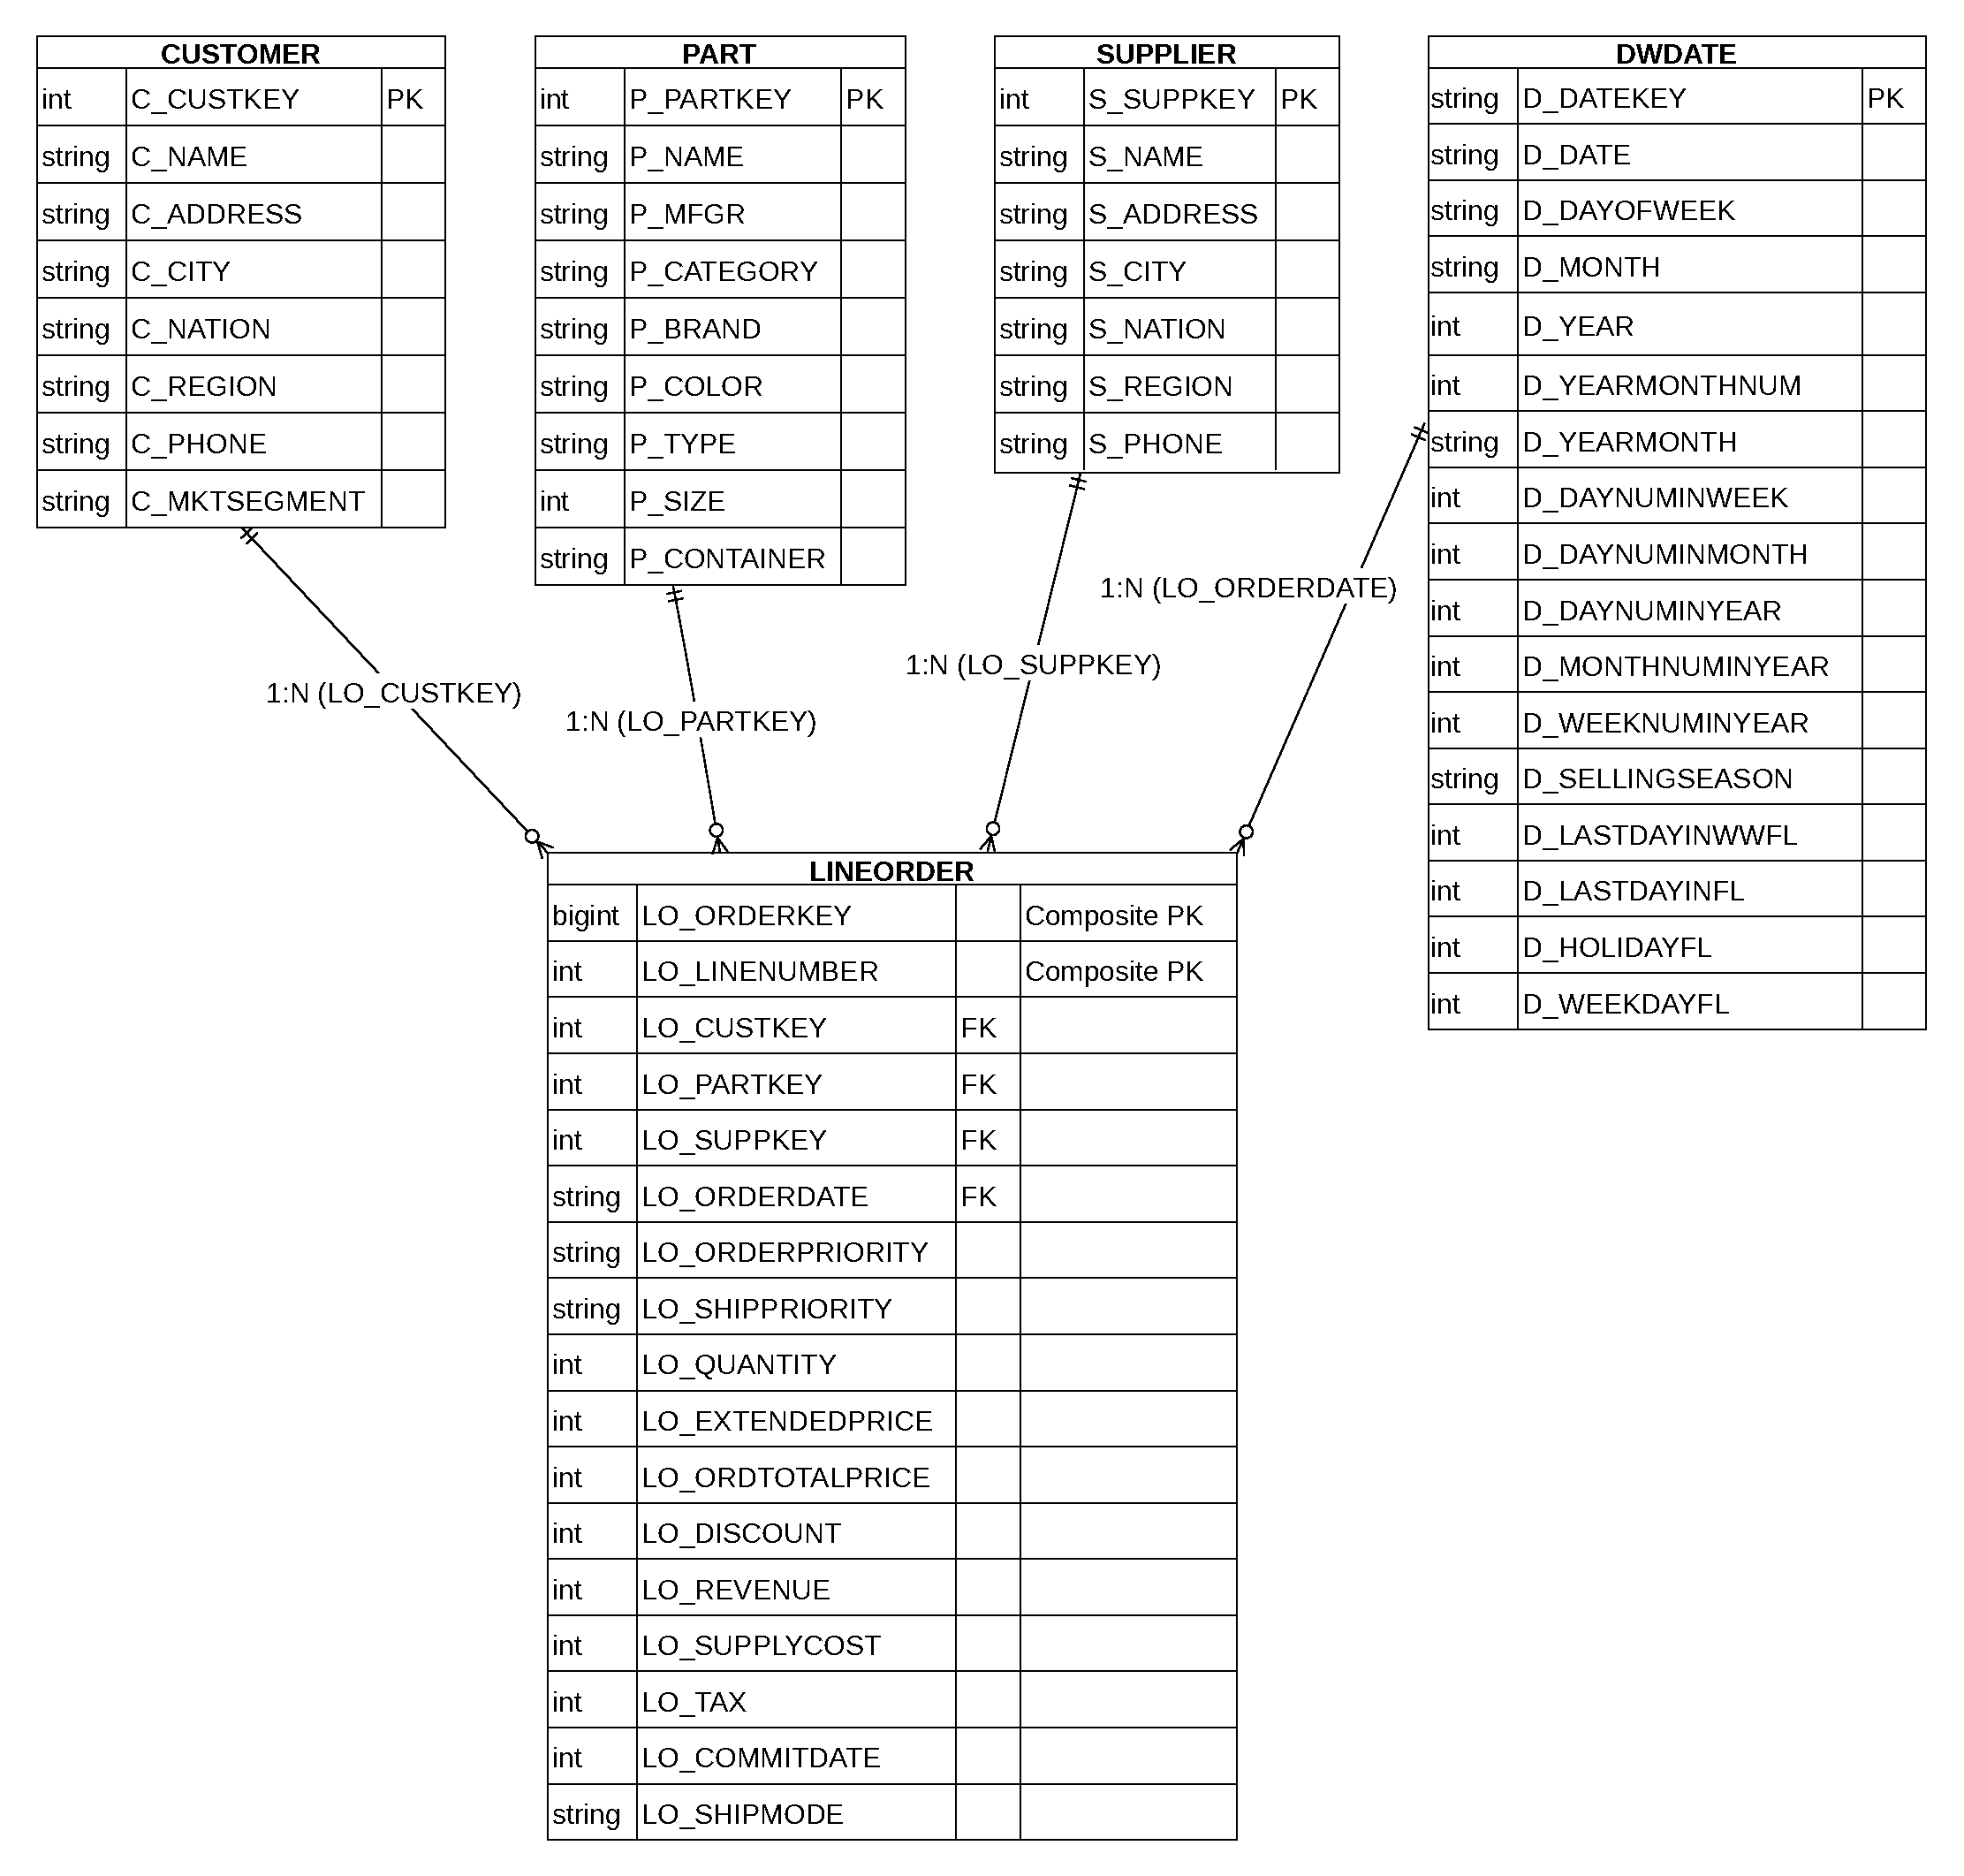
\includegraphics[width=0.85\linewidth]{content/assets/schema.pdf}
    \caption{SSB star schema entity-relationship diagram.}
    \label{fig:ssb-schema}
    
    \vspace{2em}
    
    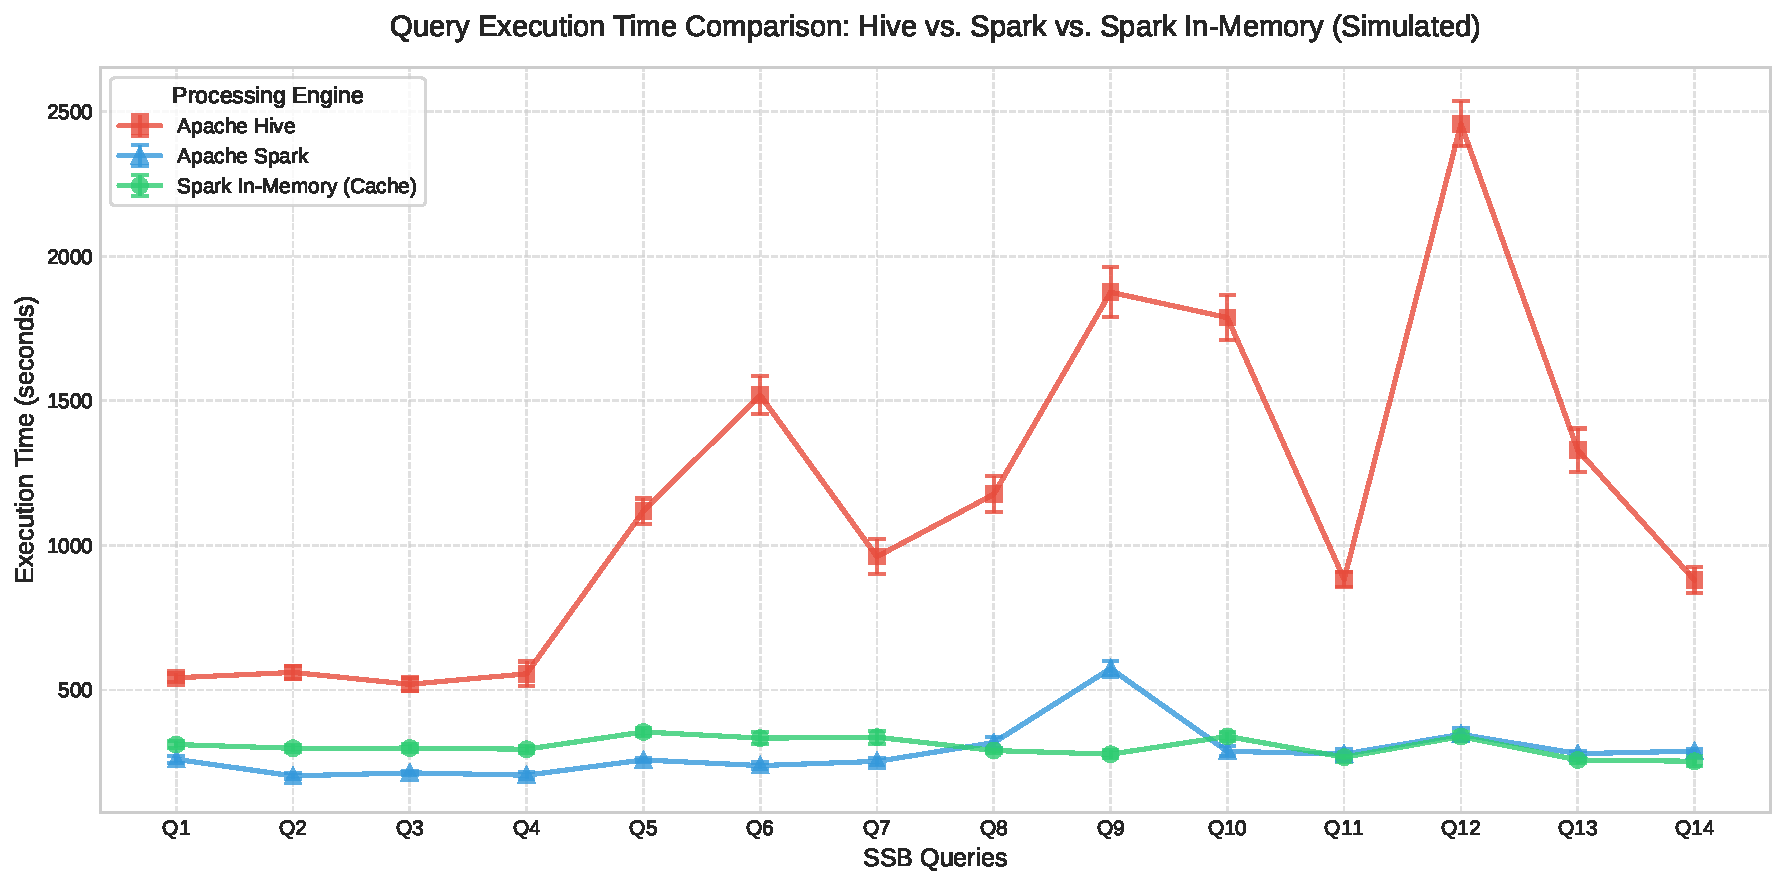
\includegraphics[width=0.85\linewidth]{content/assets/graphic.pdf}
    \caption{Query execution time comparison: Hive vs.\ Spark vs.\ Spark
             with caching.}
    % [AUTHOR VALIDATION REQUIRED: consider regenerating this figure with
    %  error bars (mean +/- SD) now that 10-iteration statistics are available.]
    \label{fig:query-execution-time-comparison}
\end{figure}

Table~\ref{tab:benchmark-results} reports the mean execution time and standard
deviation for each query across the three configurations
(Figure~\ref{fig:query-execution-time-comparison}).

\begin{table}[htbp]
  \centering
  \caption{Mean query execution time in seconds, with standard deviation in
           parentheses, over 10 iterations per configuration.}
  \label{tab:benchmark-results}
  \renewcommand{\arraystretch}{1.15}
  \small
  \begin{tabular}{@{} l c c c @{}}
    \hline
    \textbf{Query} & \textbf{Hive} & \textbf{Spark} & \textbf{Spark+Cache} \\
    \hline
    Q1  &  541.5\,(14.9) & 259.9\,(11.1) & 311.0\,(11.9) \\
    Q2  &  561.1\,(23.0) & 203.0\,\phantom{0}(9.7) & 298.7\,(11.7) \\
    Q3  &  518.8\,(21.9) & 213.0\,\phantom{0}(7.9) & 299.4\,(14.1) \\
    Q4  &  557.0\,(42.8) & 204.9\,(12.4) & 295.3\,(11.7) \\
    Q5  & 1120.2\,(44.0) & 257.8\,\phantom{0}(6.1) & 354.2\,(14.4) \\
    Q6  & 1519.3\,(65.3) & 238.2\,(10.8) & 334.0\,(20.6) \\
    Q7  &  959.4\,(59.9) & 252.5\,(13.1) & 336.2\,(22.9) \\
    Q8  & 1175.1\,(62.2) & 318.3\,(20.3) & 290.0\,\phantom{0}(9.2) \\
    Q9  & 1871.5\,(87.3) & 574.8\,(27.5) & 277.7\,(14.4) \\
    Q10 & 1785.5\,(77.8) & 288.2\,(17.1) & 338.1\,(15.2) \\
    Q11 &  884.4\,(26.7) & 278.3\,(16.7) & 268.0\,(14.8) \\
    Q12 & 2459.1\,(77.9) & 347.2\,(21.1) & 339.4\,(14.6) \\
    Q13 & 1326.0\,(75.7) & 279.0\,(10.3) & 258.2\,(12.1) \\
    Q14 &  881.0\,(45.1) & 288.1\,\phantom{0}(6.2) & 253.8\,(16.5) \\
    \hline
  \end{tabular}
\end{table}

\paragraph{Hive versus Spark.} Across all 14 queries, Spark outperformed Hive
by a mean margin of 868~seconds, with per-query differences ranging from
282~seconds (Q1) to 2\,112~seconds (Q12). The improvement is most pronounced
for multi-join queries that operate on the full \texttt{lineorder} fact table.
All differences are consistent across the 10 iterations, as indicated by the
relatively low standard deviations.

\paragraph{Spark versus Spark with caching.} The comparison between the two
Spark configurations is less straightforward. For the simpler two-join queries
(Q1--Q4) and several four-join queries (Q5--Q7, Q10), the cached configuration
was 50--97~seconds \emph{slower} than the uncached baseline. This penalty
stems from the overhead of attempting to cache the 9.3~GB \texttt{lineorder}
table into the cluster's limited memory: the table cannot be fully cached, but
the associated shuffle and spill costs still penalise execution. For the more
complex queries (Q8, Q9, Q11--Q14), partial caching of the smaller dimension
tables yielded a net benefit, with Q9 showing the largest gain (297~seconds).
Averaged across all 14 queries, the cached configuration was 18~seconds slower
than uncached Spark, indicating that caching is counterproductive under these
memory constraints unless the query complexity is sufficient to amortise the
overhead.

\paragraph{Resource constraints.} The Spark configurations were as follows:

\begin{lstlisting}[language=SQL, caption={Spark launch parameters.}, label={lst:spark-configuration}, frame=single, basicstyle=\ttfamily\scriptsize]
-- standard execution
spark-sql --master yarn
-- cached execution
spark-sql --master yarn   --num-executors 2   --executor-cores 1   --driver-memory 512m   --executor-memory 1g   --conf spark.executor.memoryOverhead=256m   --conf spark.memory.fraction=0.8   --conf spark.sql.shuffle.partitions=48
\end{lstlisting}

The restriction to two executors (\texttt{-{}-num-executors\,2}) reflects a
hard CPU constraint, not merely a memory limitation. The blueprint configures
one virtual core per NodeManager, and three of the four nodes act as
NodeManagers, yielding three YARN containers in total. Because the Spark
Application Master claims one container, at most two remain available for
executors. Any attempt to allocate a third executor would cause a resource
deadlock.

Despite these constraints, all 420 query executions (14 queries $\times$ 10
iterations $\times$ 3 configurations) completed without unrecoverable failures.
Spark fell back to disk gracefully when in-memory caching could not be
sustained, confirming the operational stability of the platform under
prolonged stress.
